\subsection{Compared with analytical result}

We started with a small two dimensional lattice with lattice size $L$=2 and at T= 1.0 $\text{k}_\text{B}T/\text{J}$ with random initial state are in Figures \ref{fig:L_2_energy}, \ref{fig:L_2_magnetic_abs}, \ref{fig:L_2_heat_capacity} and \ref{fig:L_2_susceptibility}. From the plots, we can see that the numerical result gives a good agreement with the analytical values calculated in \ref{sec:analytical_sol} Analytical solutions for L=2 after approximately $5\cdot 10^5$ Monte Carlo cycles. Table \ref{tab:compare_values} lists the result after $10^6$ Monte Carlo cycles, and it show a good agreement as well. 

\begin{table}\caption{This table compares the analytical values for $L$=2 with the numerical ones after $10^6$ Monte Carlo cycles. The values are in units per spin and at T=1.0 $\text{k}_\text{B}T/\text{J}$.}\label{tab:compare_values}
\begin{tabular}{ccc}
& Numerical: & Analytical:\\ \hline
$\left<E\right>\, [E_{kl}]$ &   -1.9958 & -1.9960\\
$\left<E^2\right>\, [E_{kl}^2]$ &   15.9664 & 15.9679\\
$\left<M\right>$ &    0.0451 & 0\\
$\left<M^2\right>$ &    3.9930 & 3.9933\\
$\left<|M|\right>$ &    0.9986 & 0.9987\\
$\chi \, [J/k_B^T]$ &   3.9849 & 3.9933\\
$C_V \, [J^2/k_B^3T^2]$& 0.0335 & 0.0321\\
\end{tabular}
\end{table}

\begin{figure}[H]
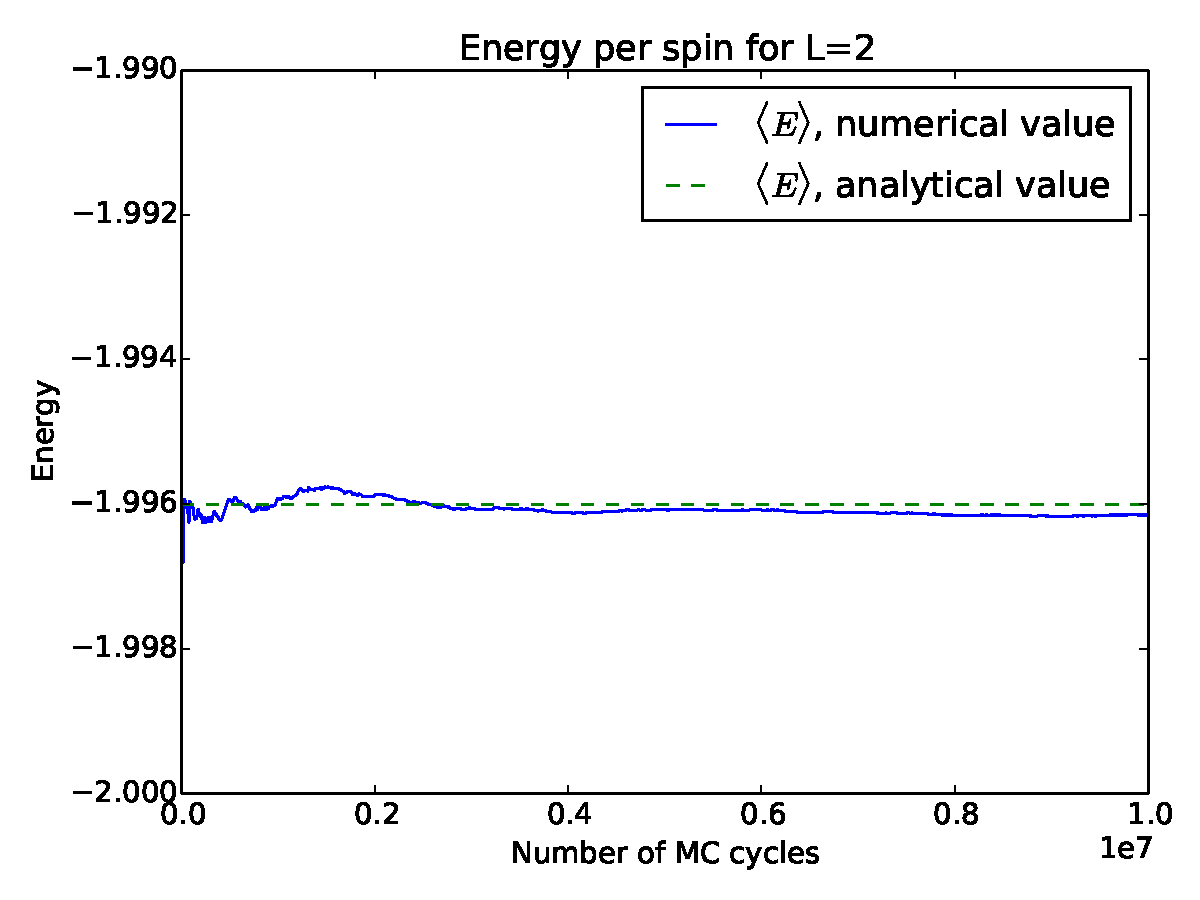
\includegraphics[width=\linewidth]{../results/4b/L_2_energy}\caption{This is a plot of the expectation value of the energy per spin verus number of Monte Carlo cycles. The plot shows that we have a good agreement after $ 5 \cdot 10^{5} $ MC cycles.}\label{fig:L_2_energy}
\end{figure}

\begin{figure}[H]
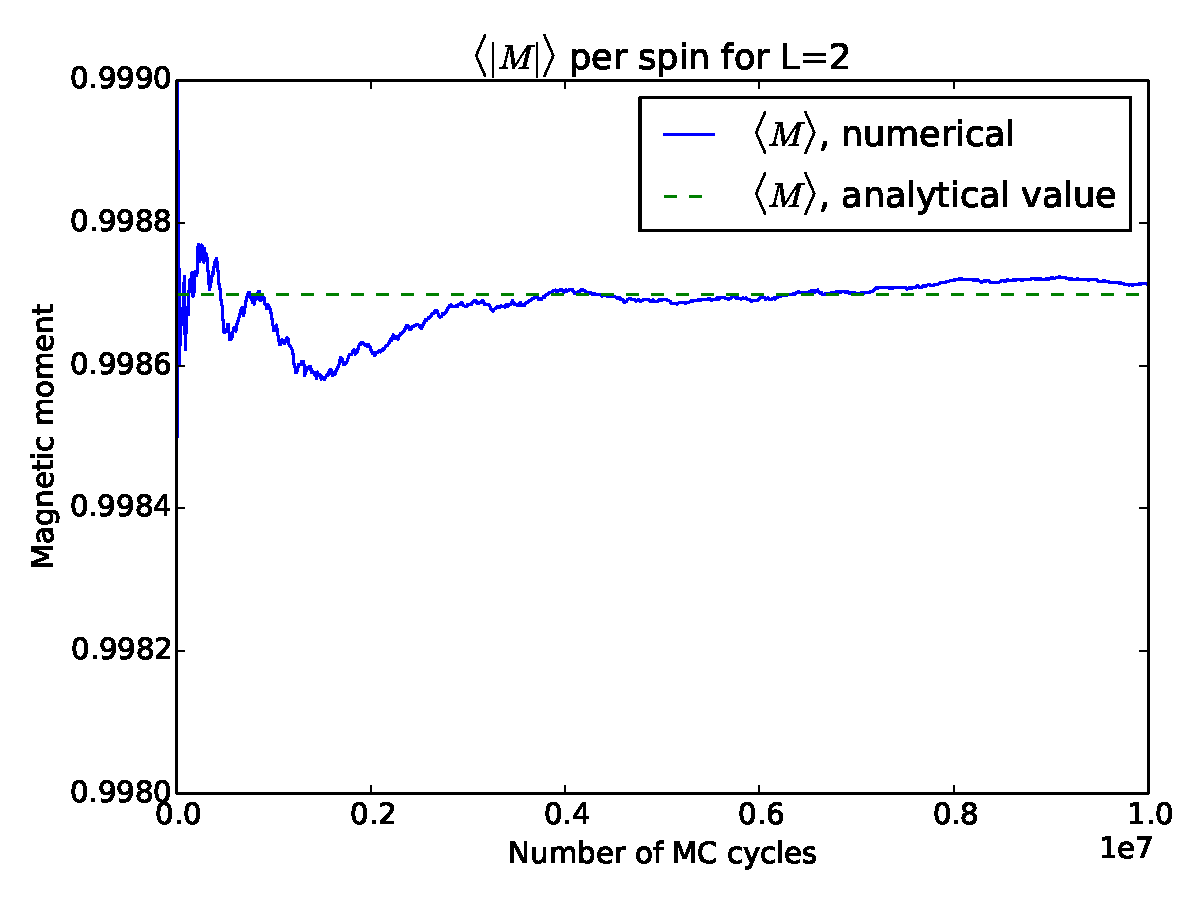
\includegraphics[width=\linewidth]{../results/4b/L_2_magnetic_abs}\caption{This is a plot of the expectation value of the mean absolute value of the magnetic moment per spin verus number of Monte Carlo cycles. The plot shows that we have a good agreement after $ 5 \cdot 10^{5} $ MC cycles.}\label{fig:L_2_magnetic_abs}
\end{figure}

\begin{figure}[H]
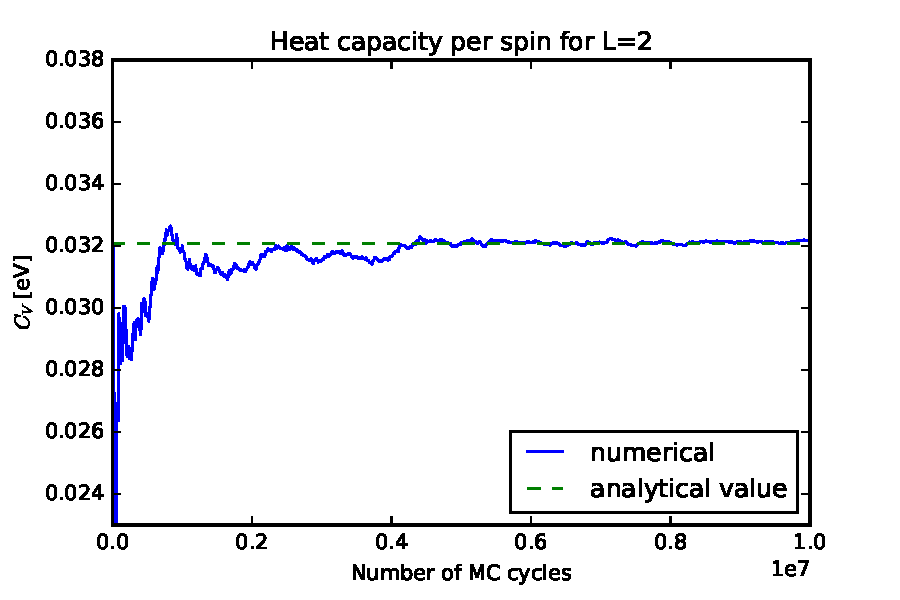
\includegraphics[width=\linewidth]{../results/4b/L_2_heat_capasity}\caption{This is a plot of the heat capacity per spin verus number of Monte Carlo cycles. The plot shows that we have a good agreement after $ 5 \cdot 10^{5} $ MC cycles.}\label{fig:L_2_heat_capacity}
\end{figure}

\begin{figure}[H]
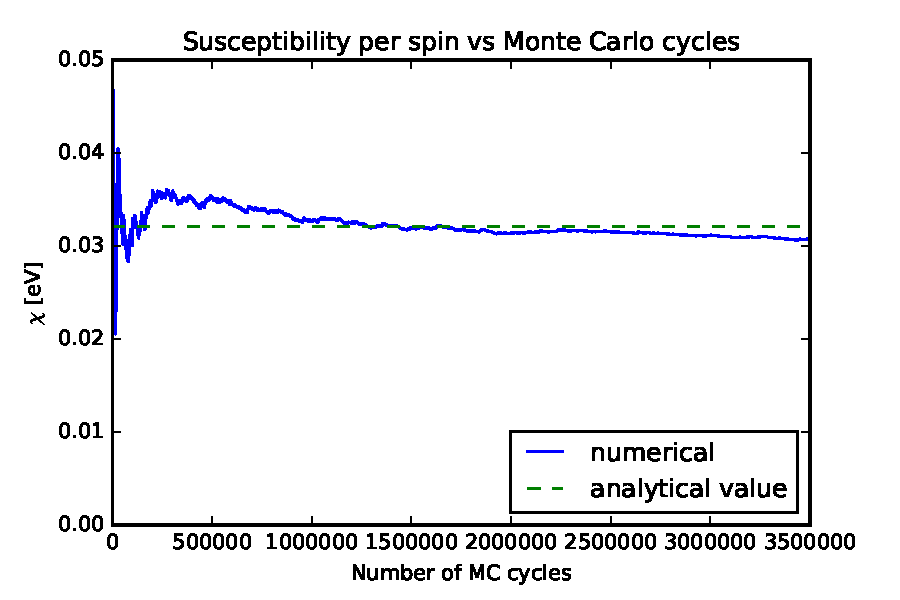
\includegraphics[width=\linewidth]{../results/4b/L_2_susceptibility}\caption{This is a plot of the susceptibility per spin verus number of Monte Carlo cycles. The plot shows that we have a good agreement after $ 5 \cdot 10^{5} $ MC cycles.}\label{fig:L_2_susceptibility}
\end{figure}

\begin{figure}[H]
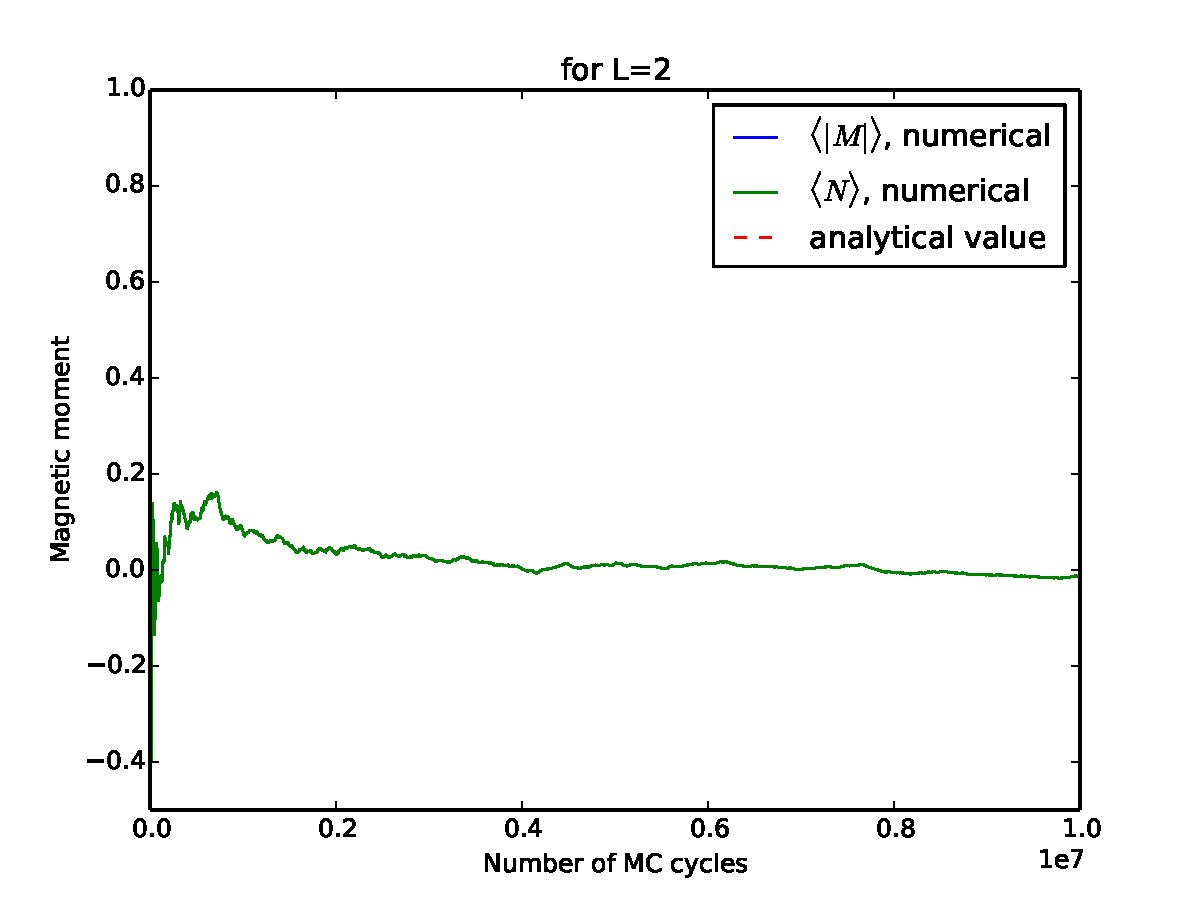
\includegraphics[width=\linewidth]{../results/4b/L_2_magnetic}\caption{This is a plot of the expectation value of the mean value of the magnetic moment per spin verus number of Monte Carlo cycles. The plot shows that we would not have had a good agreement after $ 5 \cdot 10^{5} $ MC cycles, when not using the absolute value as in Figure \ref{fig:L_2_magnetic_abs}.}\label{fig:L_2_magnetic}
\end{figure}


We see that the energy converges fastest. The magnetic moment is not converging as fast but still fast, we are plotting the absolute value, and that makes it converge faster, because the oscillation between the same size, but different signs does not show. Figure \ref{fig:L_2_magnetic} shows how the magnetic moment converges much slower. It can be shown however that the magnetic moment will converge, but slower and we would have needed more Monte Carlo cycles. 

\subsection{Equilibration time}

We increased the size of the system to $L$ = 20 and saw how both the temperature and the initial state affected the procedure by again plotting against number of Monte Carlo cycles. %From Figure \ref{fig:L_20_energy_mag_T_1.0} and Figure \ref{fig:L_20_energy_mag_T_2.4}, we can see that approximately $5\cdot 10^5$ Monte Carlo cycles is a good equilibrium time, the time the model needs to reach equilibrium. 


\subsubsection{Initial state}

\begin{figure}[H]
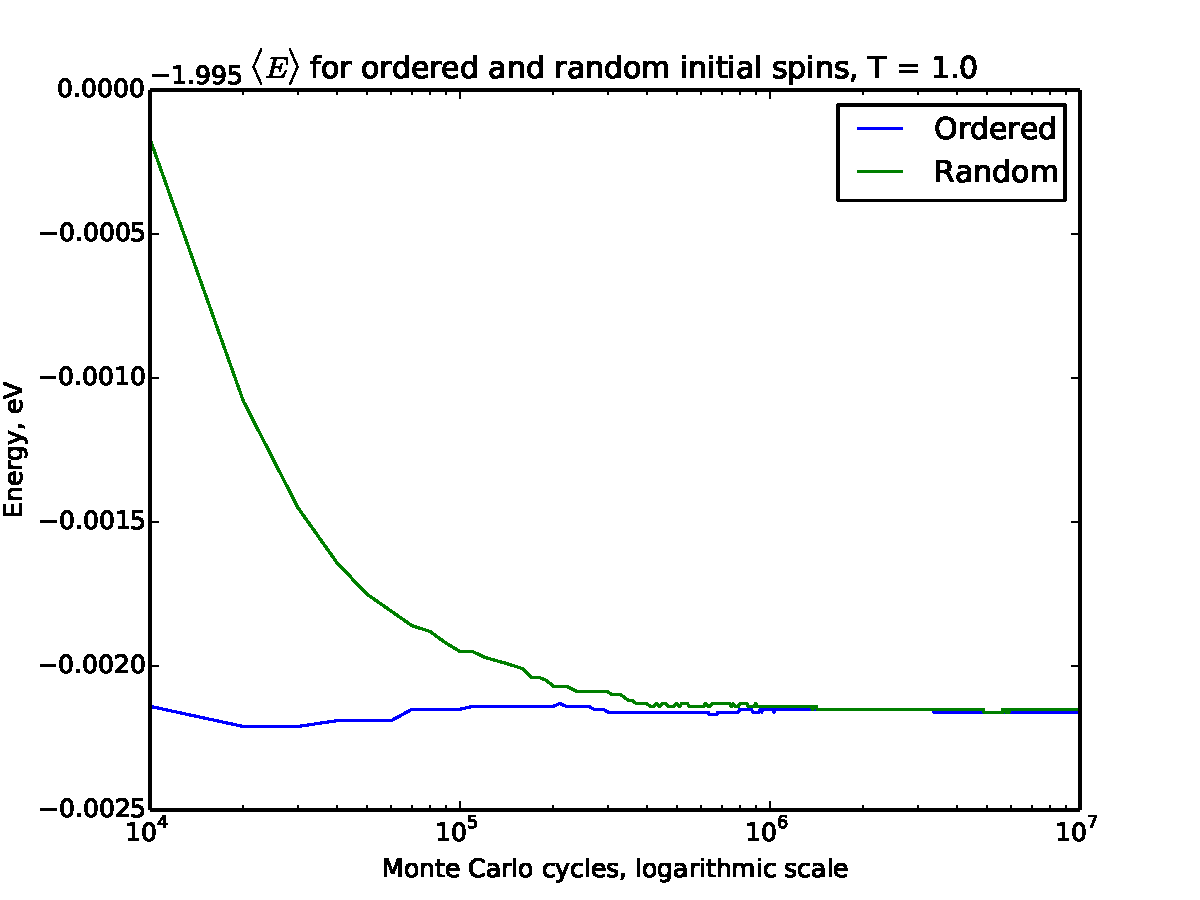
\includegraphics[width=\linewidth]{../results/4c/ran_order_T1}\caption{This is a plot of both the expectation value of the energy and absolute magnetic moment per spin verus number of Monte Carlo cycles at T = 1.0 $\text{k}_\text{B}T/\text{J}$. The plot shows the difference in the behaviour of the ordered initial state and a random initial state.}\label{fig:L_20_initial_T_1.0}
\end{figure}

\begin{figure}[H]
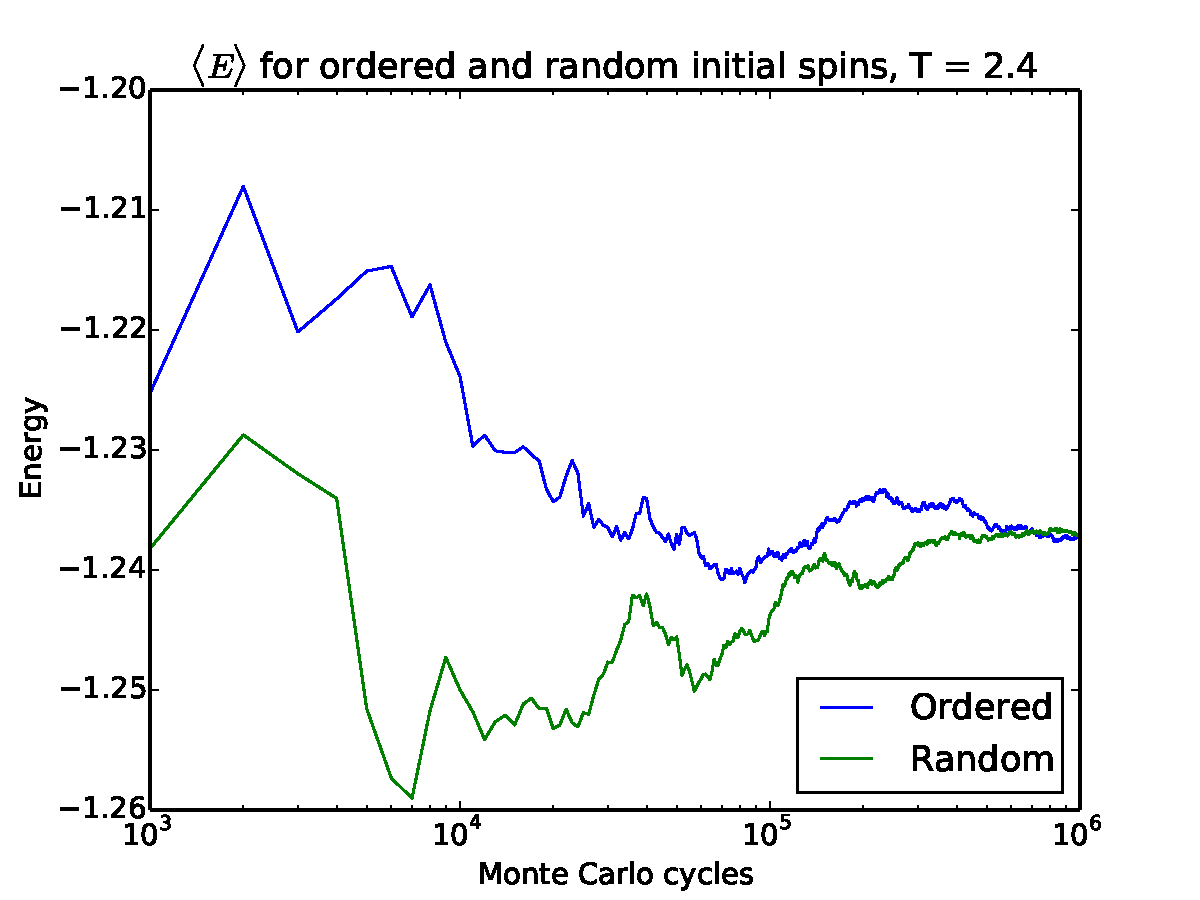
\includegraphics[width=\linewidth]{../results/4c/ran_order_T2}\caption{This is a plot of both the expectation value of the energy and absolute magnetic moment per spin verus number of Monte Carlo cycles at T = 2.4 $\text{k}_\text{B}T/\text{J}$. The plot shows the difference in the behaviour of the ordered initial state and a random initial state.}\label{fig:L_20_initial_T_2.4}
\end{figure}

Figure \ref{fig:L_20_initial_T_1.0} compares the development of the expectation value for the energy with an ordered initial state, all spin up, and a random initial state at the temperature 1.0 $\text{k}_\text{B}T/\text{J}$. We see from the plot that the ordered initial state converges much earlier. This might be because the ordered state reflects the most likely state, better then the random state, at small temperatures.

Figure \ref{fig:L_20_initial_T_2.4} shows the same for the temperature 2.4 $\text{k}_\text{B}T/\text{J}$. We see from the plot that the two initial states act similarly and converges similarly. They do not converge as at low temperature, but that is expected because of the increase in temperature.

Because the random initial state converged slower then the ordered one, we compared the random initial states when we looked at both the magnetic moment and the energy at the two temperatures and found an equilibrium time.

\subsubsection{Different temperatures}


\begin{figure}[H]
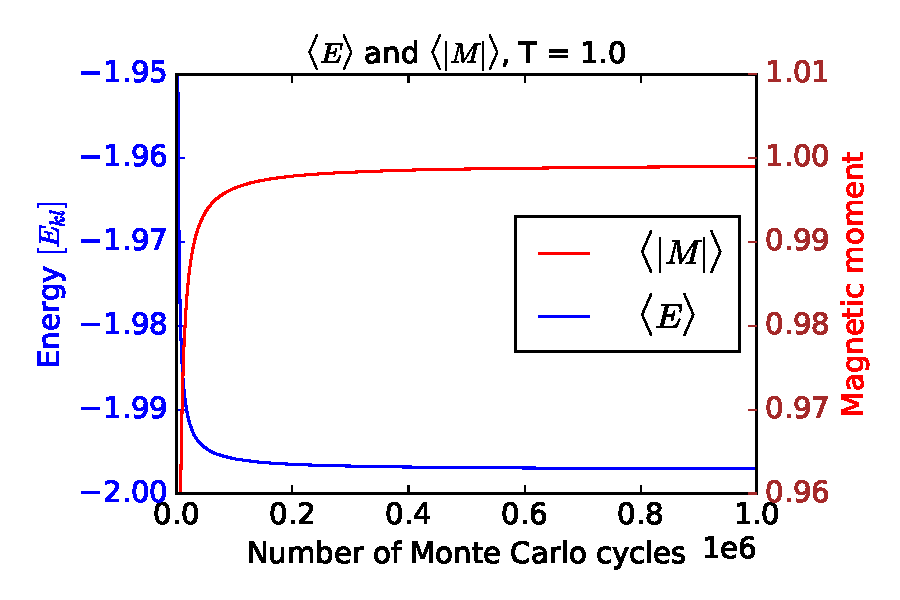
\includegraphics[width=\linewidth]{../results/4c/En_mag_T1_0}\caption{This is a plot of both the expectation value of the energy and absolute magnetic moment per spin verus number of Monte Carlo cycles at T' = 1.0 $\text{k}_\text{B}T/\text{J}$. The plot shows that an equilibrium is reached already at $2 \cdot 10^{5}$ MC cycles.}\label{fig:L_20_energy_mag_T_1.0}
\end{figure}

\begin{figure}[H]
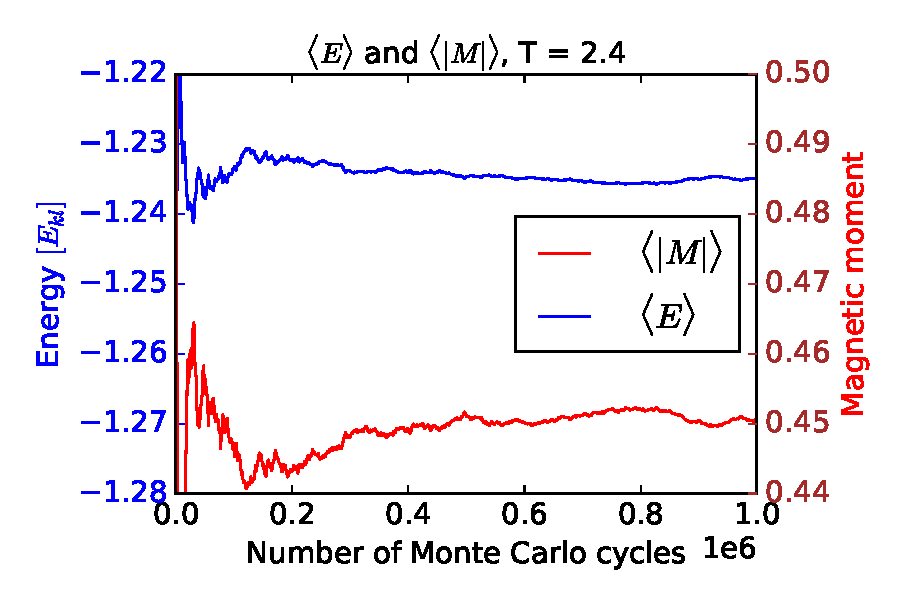
\includegraphics[width=\linewidth]{../results/4c/En_mag_T2_4}\caption{This is a plot of both the expectation value of the energy and absolute magnetic moment per spin verus number of Monte Carlo cycles at T = 2.4 $\text{k}_\text{B}T/\text{J}$. The plot shows that an equilibrium is reached at around $5 \cdot 10^{5}$ MC cycles.}\label{fig:L_20_energy_mag_T_2.4}
\end{figure}


Figure \ref{fig:L_20_energy_mag_T_1.0} and Figure \ref{fig:L_20_energy_mag_T_2.4} shows the result for $L$ = 20 at two different temperatures and give different equilibration times. Figure \ref{fig:L_20_energy_mag_T_1.0} shows that the values are $\pm 0.005$ from the equilibrium values already at $2\cdot 10^5$ Monte Carlo cycles, but if we want even better accuracy, we need to wait till $5\cdot 10^5$ Monte Carlo cycles. If we look at Figure \ref{fig:L_20_energy_mag_T_2.4} though, we see that the values are $\pm 0.005$ from the equilibrium values from around $5\cdot 10^5$ Monte Carlo cycles.

The equilibration time is then approximately $5\cdot 10^5$ Monte Carlo cycles at T' = 2.4 $\text{k}_\text{B}T/\text{J}$ and lower for the lower temperature, so $5\cdot 10^5$ that is what we used when we counted the energies to get the probabilities. 

\begin{figure}[H]
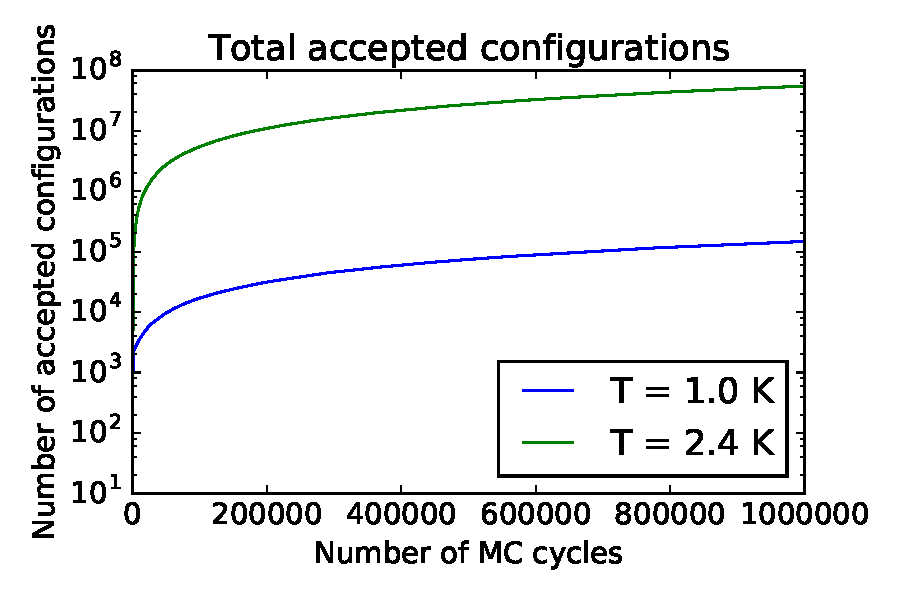
\includegraphics[width=\linewidth]{../results/4c/L_20_total_accepted}\caption{This is a plot of the total number of accepted configurations versus number of Monte Carlo cycles with random initial state.}\label{fig:total_accepted}
\end{figure}

The values are fluctuating a lot more when the temperature is higher. Figure \ref{fig:total_accepted} shows the total number of accepted configurations with increasing number of Monte Carlo cycles. It is easy to see that the algorithm accepts more configurations when the temperature is higher. It not that easy to see, since it is a logarithmic plot, but the slope of the higher temperature one is larger then the lower temperature one, after equilibrium. This is also what we see with the fluctuations in the expectation plots. This is what we will look into in \ref{sec:probability} Energy probability.


%\begin{figure}[H]
%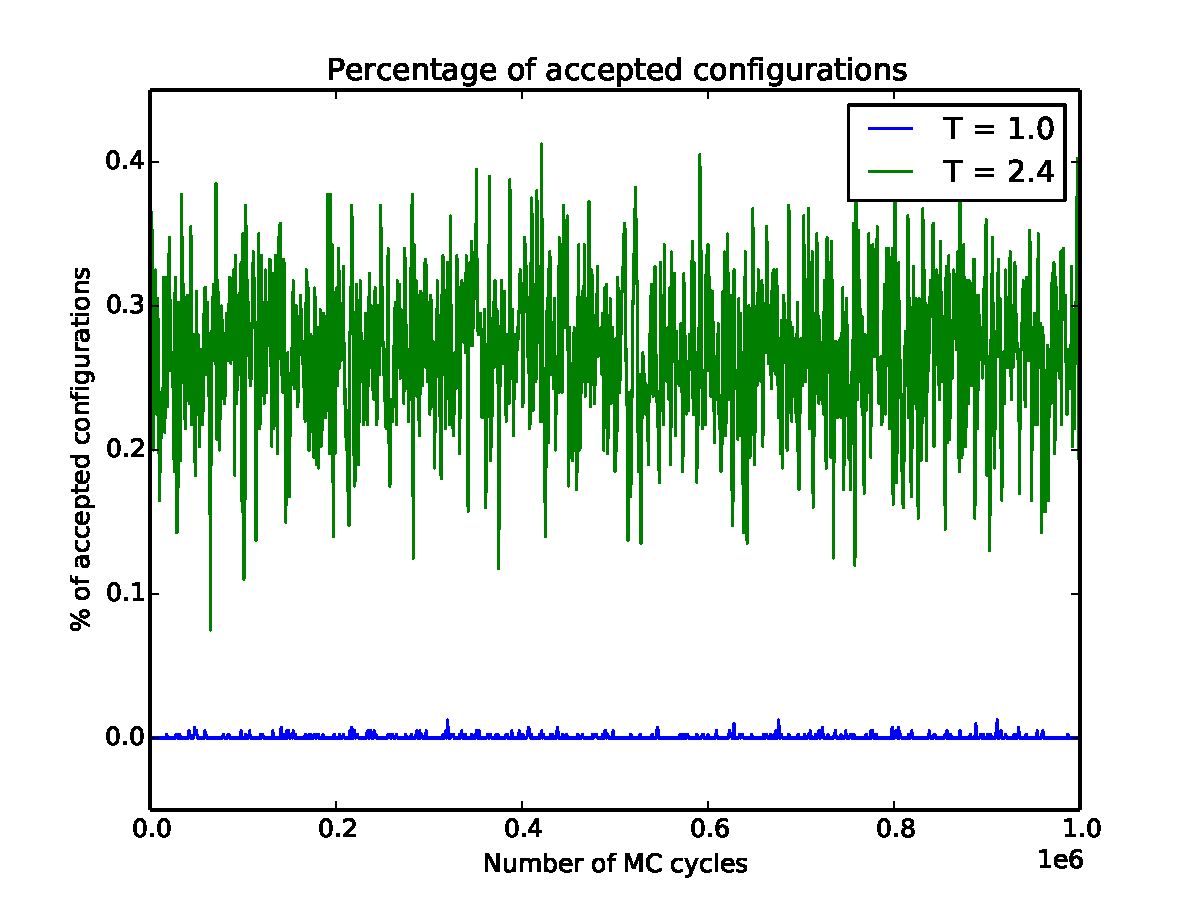
\includegraphics[width=\linewidth]{../results/4c/L_20_accepted_configs}\caption{This is a plot of the percentage accepted of attempted configurations versus  Monte Carlo cycles with random initial state.}\label{fig:percentage_accepted}
%\end{figure}

\subsection{Energy probability}\label{sec:probability}

\begin{figure}[H]
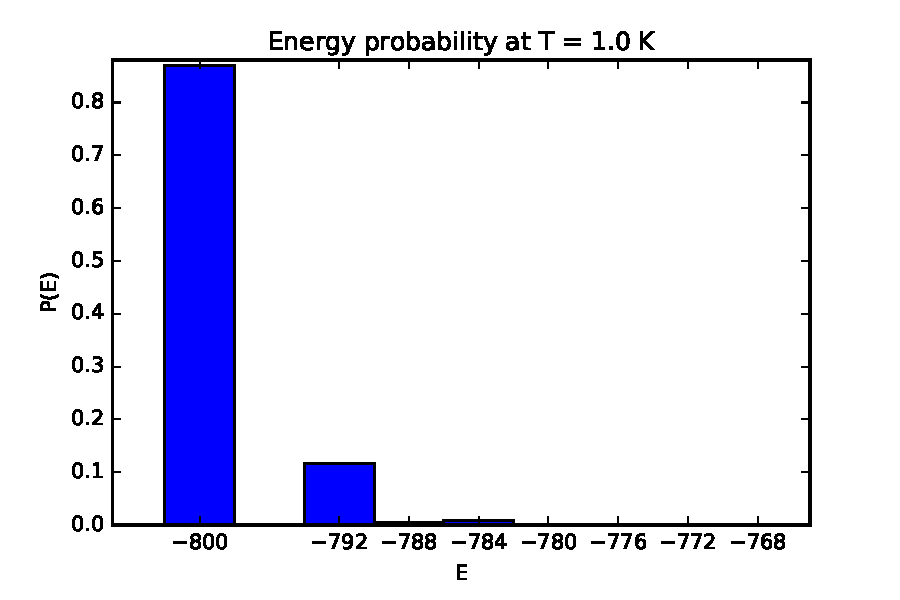
\includegraphics[width=\linewidth]{../results/4d/d_T_1probability}\caption{This is a plot of the energy probability when T' = 1.0 $\text{k}_\text{B}T/\text{J}$. The energy is the total energy of the 2D lattice with $20\times 20$ spins.}\label{fig:probability_T_1.0}
\end{figure}

\begin{figure}[H]
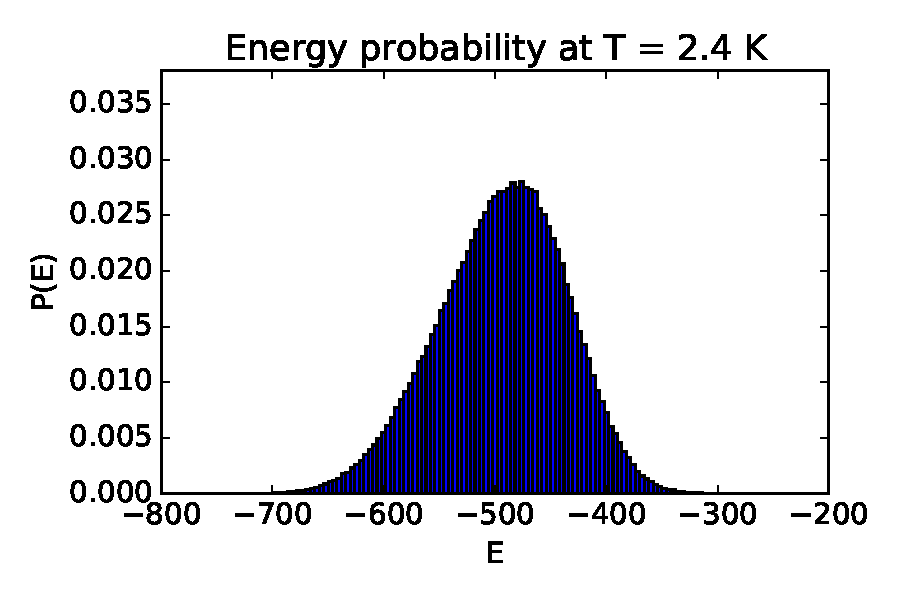
\includegraphics[width=\linewidth]{../results/4d/d_T_2_4probability}\caption{This is a plot of the energy probability when T' = 2.4 $\text{k}_\text{B}T/\text{J}$.The energy is the total energy of the 2D lattice with $20\times 20$ spins.}\label{fig:probability_T_2.4}
\end{figure}

Figure \ref{fig:probability_T_1.0} shows the probability density of the energy at T' = 1.0 $\text{k}_\text{B}T/\text{J}$. The graph reflects the little fluctuation in the expectation values. Figure \ref{fig:probability_T_2.4} however, shows that with higher temperature the probability density is more smeared out around the most likely state. 

This fits with the Boltzmann distribution (Equation \ref{eq:Boltzmann}). The difference in temperature changes the probability of accepting transition moves (Equation \ref{eq:acceptance}) 'away' from the most likely state, $ \Delta E_{ij} > 0$:
\[
e^\frac{-\Delta E_{ij}}{k_B T_1} > e^\frac{-\Delta E_{ij}}{k_B T_2}\hspace{1cm}\text{if } T_1 > T_2
\]

We calculated the variance to compare it with the probability plots in Figures \ref{fig:probability_T_1.0} and \ref{fig:probability_T_2.4}:

The variance of the energy is given by:
$$ \sigma_E^2 = \left< E^2\right> - \left< E\right>^2 $$
and the standard deviation is $\sigma = \sqrt{\sigma^2}$.

The connection between full width half maximum (FWHM) and standard deviation can be put as: 
$$\text{FWHM} = 2 \sqrt{2ln2} \sigma \approx 2.355 \sigma$$ 
for a standard distribution \cite{FWHM}. We will use it as a guide when comparing the graphs with the variance.

T' = 1.0 $\text{k}_\text{B}T/\text{J}$:
$$ \sigma_E^2 = 638181 - (-798.855)^2 = 11.69 $$
$$ \sigma = 3.42 $$
$$ \text{FWHM} \approx 2.355 \cdot 3.24 = 7.63 $$

It is difficult to read out a FWHM from the histogram in Figure \ref{fig:probability_T_1.0} because of the few different energies. We might say it is around 10 if we assume it is symmetric. It fits alright with the calculated value. 

T' = 2.4 $\text{k}_\text{B}T/\text{J}$:
$$ \sigma_E^2 =   247886 - (-494.628)^2 = 3229.14 $$
$$ \sigma = 56.8  $$
$$ \text{FWHM} \approx 2.355 \cdot 56.8 = 133.76 $$

It is easier to read out the FWHM from Figure \ref{fig:probability_T_2.4}. We could say it is around (560-440 =) 120, and that is around what we got.

The most important point is that the variance is much larger for larger temperatures. 

\subsection{The Critical Temperature}

At last we ran the program for even bigger lattice sizes and a temperature interval, to investigate the critical temperature and the phase transition.

\begin{figure}[H]
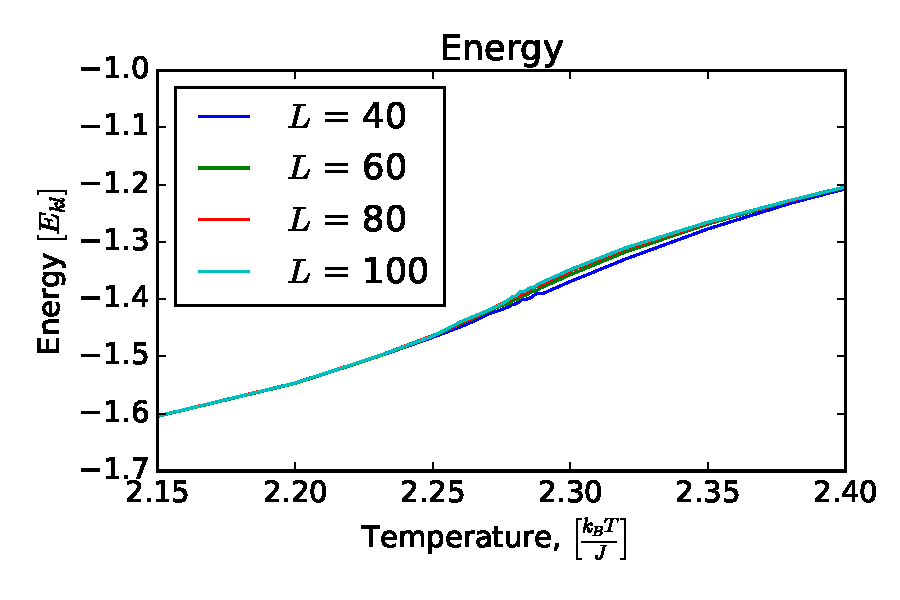
\includegraphics[width=\linewidth]{../results/4e/4e_energy}\caption{This is a plot if the energy versus temperature around the critical temperature for the different lattice sizes with $L$ = 40, $L$ = 60, $L$ = 80 and $L$ = 100.The small fluctuations are due to higher resolution in temperature around the critical temperature.}\label{fig:4e_energy}
\end{figure}

\begin{figure}[H]
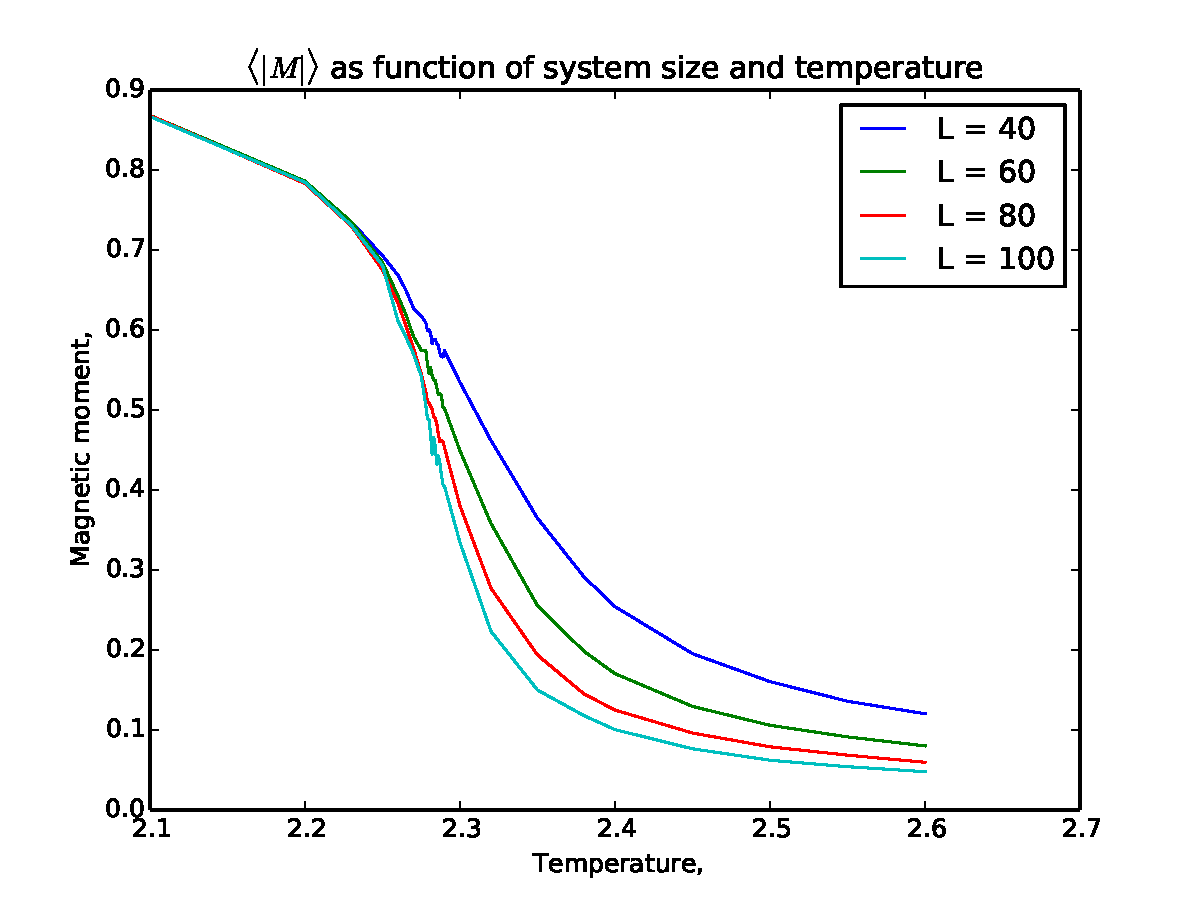
\includegraphics[width=\linewidth]{../results/4e/4e_mag}\caption{This is a plot if the absolute magnetic moment versus temperature around the critical temperature for the different lattice sizes with $L$ = 40, $L$ = 60, $L$ = 80 and $L$ = 100. The small fluctuations are due to higher resolution in temperature around the critical temperature.}\label{fig:4e_magnetic}
\end{figure}

Figure \ref{fig:4e_energy} shows energy as a function of temperature. We can see a change in the behavior around T' = 2.25-2.30 $\text{k}_\text{B}T/\text{J}$. This disturbance in the function might indicate a phase transition. The different sizes have the same behavior, but we can see that the slope is larger the larger the lattice, in the area of the supposed phase shift.

In Figure \ref{fig:4e_magnetic}, which shows the temperature dependence of the absolute value of the magnetic moment, there is a clearer change around T' = 2.30 $\text{k}_\text{B}T/\text{J}$. The change is more abrupt with larger lattice sizes. The figure does indicate that we have a phase transition from a ferromagnet with magnetic moment per spin around 0.9 to a paramagnet with magnetic moment per spin around 0. We see also here that the change is more abrupt for larger lattice sizes. The tendency shows that an infinite two dimensional lattice might give an infinite steep slope at the critical temperature. 

\begin{figure}[H]
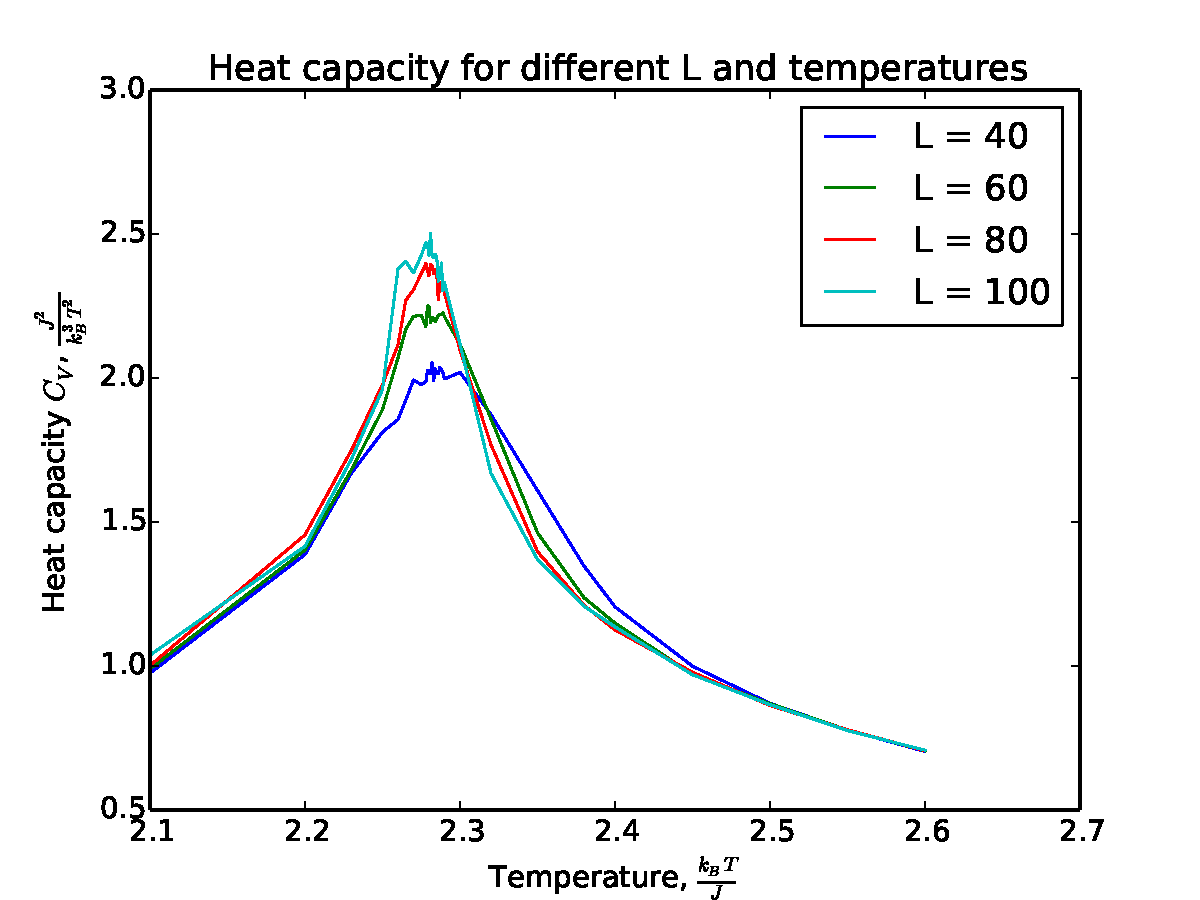
\includegraphics[width=\linewidth]{../results/4e/4e_Cv}\caption{This is a plot if the heat capacity versus temperature around the critical temperature for the different lattice sizes with $L$ = 40, $L$ = 60, $L$ = 80 and $L$ = 100. The small fluctuations are due to higher resolution in temperature around the critical temperature.}\label{fig:4e_heat_capa}
\end{figure}

\begin{figure}[H]
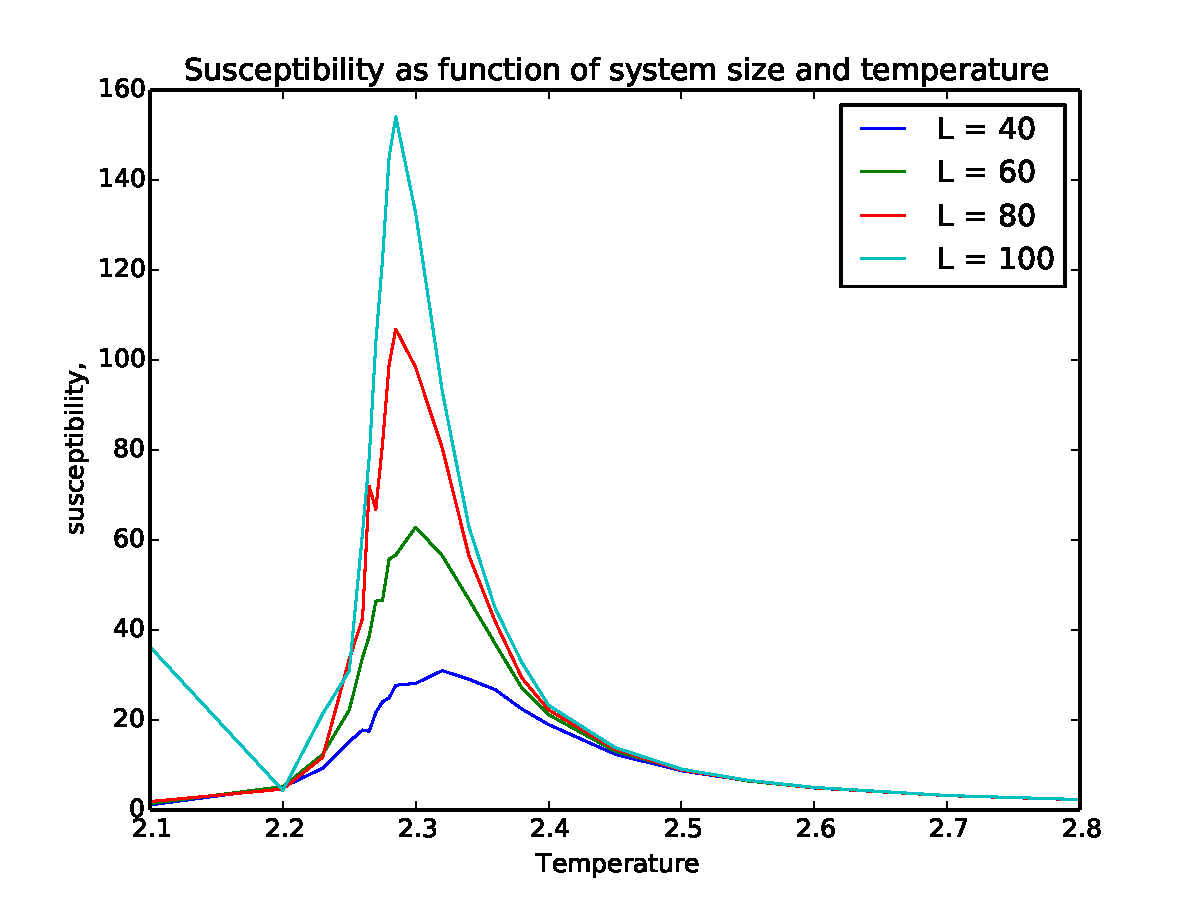
\includegraphics[width=\linewidth]{../results/4e/4e_x}\caption{This is a plot if the susceptibility versus temperature around the critical temperature for the different lattice sizes with $L$ = 40, $L$ = 60, $L$ = 80 and $L$ = 100. The small fluctuations are due to higher resolution in temperature around the critical temperature.}\label{fig:4e_suscept}
\end{figure}

Figure \ref{fig:4e_heat_capa} shows the temperature dependency of the heat capacity. The heat capacity should diverge for a second order phase transition, due to the infinite steep slope in the energy because it is the derivative of the energy with respect to temperature. We see from the plot that the peak becomes higher when the lattice size increases, and it looks like it will diverge for an infinite big lattice.

The temperature dependency of the susceptibility shows the same tendency as the heat capacity. It should diverge as well when $T' \rightarrow T_C$ because of its inverse temperature dependency (Equation \ref{eq:mag_suscept_T}).

At last we used Equation \ref{eq:critical_T} to extract $T_C (L = \infty)$.

Getting these equations from \ref{eq:critical_T} where $\nu = 1$:

From Figure \ref{fig:4e_heat_capa} we read out the $T_C(L)$ for $L$ = 40, $L$ = 60, $L$ = 80 and $L$ = 100. We used the result to do a linear regression for $T_C(L) = a\cdot L^{-1} + T_C(\infty)$ and find $T_C(\infty)$. The result is in Figure \ref{fig:linfit}. $T_C(\infty)$ was found to be 2.278 $\text{k}_\text{B}T/\text{J}$. The result is not so bad compared with the exact value $T_C(\infty) = 2/ \ln(1+\sqrt{
2}) \approx 2.269$ $\text{k}_\text{B}T/\text{J}$ \cite{Onsager}.

\begin{figure}[H]
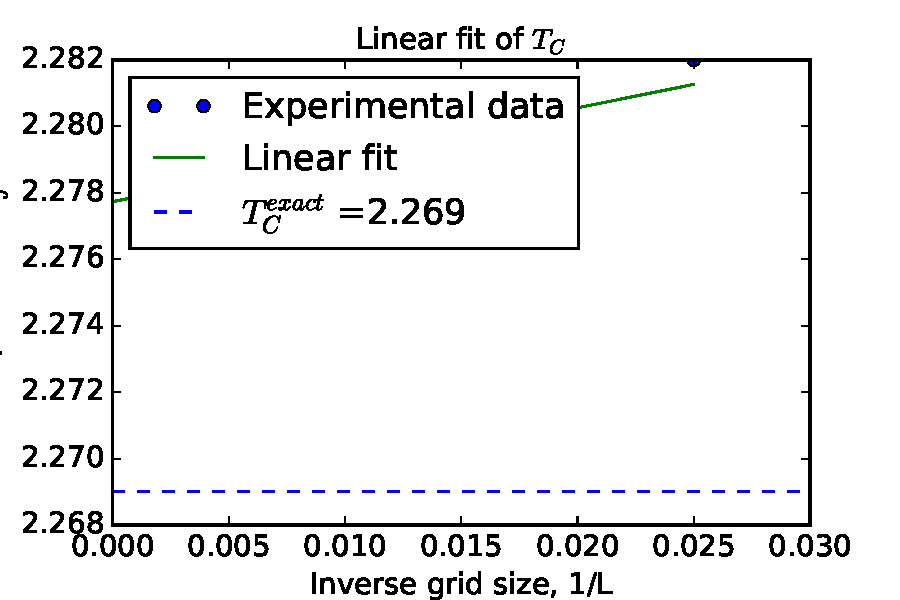
\includegraphics[width=\linewidth]{../results/4e/linfit}\caption{This plots show the points for $L$ = 40, $L$ = 60, $L$ = 80 and $L$ = 100 with their $T_C$s read of the plots of their temperature dependence (Figures \ref{fig:4e_energy} to \ref{fig:4e_suscept}). A linear regression was done on the points to find the critical temperature for $L = \infty$. The result was $T_C(\infty) = 2.278$ $\text{k}_\text{B}T/\text{J}$. }\label{fig:linfit}
\end{figure}

\subsection{CPU time}

The last thing we did was to see how the parallelization affected the CPU time. Table \ref{tab:CPU} shows the result of the timing with different number of processes.

\begin{table}\caption{This is a list of the CPU time with different numbers of processes for $L$=60 and number of Monte Carlo cycles were $10^6$.}\label{tab:CPU}
\begin{tabular}{cc}
Number of processors:& CPU time [s]: \\ \hline
 1 & 513.069\\
 2 & 306.975\\
\end{tabular}
\end{table}